We discuss the optimization opportunities and challenges through the following example. We also provide the readers a more practical example of 3 queries taken from the TPC-DS benchmark \cite{tpcds} in Section \ref{sec:tpcds-sharing}.

\begingroup
\fontsize{8pt}{9pt}
\selectfont
\begin{verbatim}
QUERY 1:
SELECT name, dept_name, salary
FROM employees, departments, salaries
WHERE dep = dept_id
	AND id = emp_id
	AND gender = 'F'
	AND location = 'us'
	AND salary > 20000
ORDER BY salary DESC

QUERY 2:
SELECT name, dept_name, title, 
	to as title_expired_on
FROM departments, employees, titles
WHERE dep = dept_id
	AND id = emp_id
	AND gender = 'F'
	AND location = 'us'
	AND salary > 20000
GROUP BY title
ORDER BY to

QUERY 3:
SELECT id, name, salary, from_date
FROM employees, salaries
WHERE id = emp_id
	AND age > 30
	AND SALARY > 30000
\end{verbatim}
\endgroup

\begin{figure*}[htbp]
	\centering
	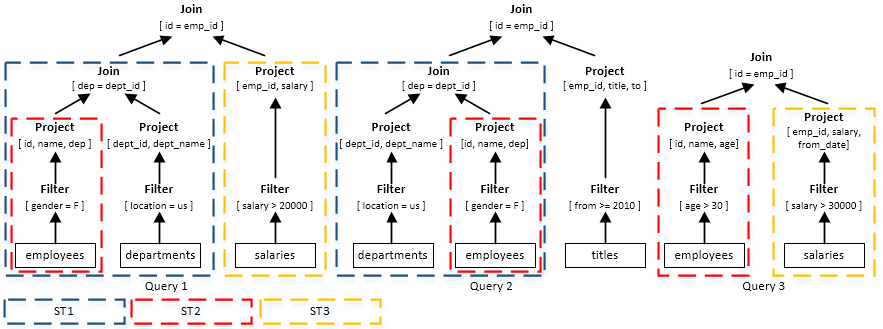
\includegraphics[scale=0.65]{figures/common_sub}
	\caption{Optimized operator trees} 
	\label{fig:common_sub}
\end{figure*}

Looking at the \emph{FROM} statements above, we can see that 3 queries (jobs) can share the common reading of \textbf{employees}, \textbf{departments} and \textbf{salaries} tables. Although disk speed has increased recently, a possible optimization would be to avoid wasteful disk I/O. Indeed, I/O operations are heavyweight because they not only involve reading records from file, but also parsing and transforming those into objects in memory for processing. What if we could tell the first job to \emph{cache} the input data after reading it, so that the later jobs do not have to ``waste time'' doing redundant I/O operations? A more refined approach could be to find common work (similar subexpressions) among these queries (for instance reading input, filtering and projecting records, joining tables, etc.) so that we can assure we are ``maximizing'' sharing benefit while ``minimizing'' the cache size (memory utilization).

To facilitate reader's understanding, we use Figure \ref{fig:common_sub} which illustrates the optimized operator trees (optimized logical plans) of the 3 queries in the above example. Those optimized logical plans are produced by Spark SQL's query optimizer that will be next translated into physical plans for execution. The leaf nodes represents the base relations. Each intermediate node is a relational algebra operator (Filter, Project, Join, etc.). The arrows indicate data flow.

As can be seen from Figure \ref{fig:common_sub}, multiple SEs can be identified. They have the same tree structure but different filtering predicates and projections, for example the similar subexpression 1 (SE1): $Project_p(Filter_f(employees))$ which appears in both 3 queries. We can save some reading, parsing, filtering and projecting costs on the \textbf{employees} table 2 times out of 3. In order to achieve that, a CE will be constructed by ``combining'' operators' predicates: \[Project_{id, name, dep, age}(Filter_{gender=F \cup age>30}(employees))\]

Constructing the CE in this way makes its output can be used to answer the consumer queries. By executing this CE and keeping the result in memory, the consumers can retrieve that data instead of reading and computing again from scratch. Thereby, the query execution time reduces significantly. Imagine that the Projection operator only projects on 4 out of total 10 columns and the Filtering keeps 60\% of records in \textbf{employees} tables, then the consumers rather than re-read and scan the whole table from disk, they can just extract from a smaller chunk of cached data in-memory. 

In the same way, the SE2 share the projection and filtering on \textbf{salaries} table. A possibly better sharing option is to let the 3 queries share the greater SEs at ($Project_2$, $Project_7$, $Project_{12}$) so that they will even further benefit from the cost of joining 2 tables \textbf{date dim} and \textbf{store sales}. Furthermore, query 3 and query 55 could share the greatest SEs at ($Project_1$, $Project_6$), joining 3 tables \textbf{date dim}, \textbf{store sales} and \textbf{item}. However, sharing greater SEs is not always better than sharing smaller ones. Specifically in this example, what if the \emph{Join} operator produces a large amount of data that is too expensive to \emph{cache} under a limited amount of memory resource? Note that data caching in memory can be a costly operation, especially in distributed environment. Our study shows that blindly caching data may lead to higher costs of job execution. One next problem we may have to face is to select multiple CEs that will later become multiple \emph{cache plans} such that the job's performance is maximized while the memory consumption condition is satisfied.

Hence, the problem we attempt to solve in this paper can be described as follows: Given a batch of queries submitted, transform it into a more efficient batch such that the new batch results in shorter aggregate job running time, taking into account the memory constraint and extra computations. Particularly in this work, we develop the solution of automatically determining the best cache plans to achieve work sharing for Spark SQL queries. It is the purpose of following sections to first demonstrate and then evaluate our unified solution for an in-memory cached-based work sharing for large-scale distributed systems.